\documentclass[../root.tex]{subfiles}

\begin{document}

\section{MDPs and SSPPs}

The concepts of MDPs (\emph{Markov Decision Process}) and SSPPs
(\emph{Stochastic Shortest Path Problem}) are a fundamental
part of this work. The reason is that we want to account for probabilistic
actions and they allow to model such stochasticity.
The implemented determinization methods described in
Chapter~\ref{chap:determinization} are meant to solve efficiently MDPs in an
on-line manner. Therefore, in order to fully understand them, we present
here the formal definition of MDPs and SSPPs. We focus on discrete MDPs
formulations. Notice that it is possible to consider continuous state
and/or actions spaces, although these naturally present more challenges.

\theoremstyle{definition}
\begin{definition}{\bfseries Markov Decision Process}
	A Markov Decision Process is a tuple $ (S, A, T, R, \gamma) $ where:
	\begin{itemize}
		\item $ S $ is a finite set of states.
		\item $ A $ is a finite set of actions.
		\item $ T(s,a,s') = \mathbb{P}(S_{t+1} = s' | S_t = s \land A_t=a) $ is
		a probabilistic Markov transition model. For each triplet
		$ (s, a, s') $, it indicates the probability of transitioning from $ s $
		to $ s' $ when action $ a $ is taken in state $ s $.
		\item $ R(s,a,s') $ is a reward function where $ R(s,a) $ is the immediate
		reward for transitioning from state $ s $ to state $ s' $ through $ a $.
		\item $ \gamma $ is the discount factor. Rewards are diminished
		by this factor after each time step.
	\end{itemize}
\end{definition}

There are alternative
definitions that consider a reward of the form $ R(s) $, and also of
the form $ R(s,a) $. These can be made
equivalent with a slight re-parametrization of the problem. They
do not alter the problem in any fundamental way~\cite{russell2016artificial}.

The reward accumulated over time is:
\[ \sum_{t=0}^\infty \gamma^t R(s_t, a_t, s_{t+1}) \],
where $ a_t $ is the action selected by the agent at each time step.
Solving a MDP consists in finding a \emph{policy} that maximizes the total or accumulated
reward. A policy is a function $ \pi (s) \in A $ that maps each state
to the action that the agent should preferentially use in that state.

The discount factor $ \gamma $ gives or subtract importance
to the long-term reward. A very low $ \gamma $ may result in a process in which
only the most immediate and short-term actions have an effect in the
accumulated reward. $ \gamma < 1 $ is very convenient because it guarantees
that the accumulated reward is bounded, as long as all the immediate rewards
are not infinite. $ \gamma = 0.99 $ and $ \gamma = 0.95 $ are usual choices.

We can assign an utility function to each state. This function gives an
idea of the accumulated reward that we can expect to obtain if this state
is reached. This utility function is defined as a \emph{Bellman equation}:
\[ V(s) = \max_a \left\{ \sum_{s'} \left( R(s, a, s') + \gamma \mathbb{P}(S_{t+1} = s' | S_t = s \land A_t=a) V(s') \right) \right\} \].

This equation already gives an indication for a couple of dynamic programming
algorithms for solving MDPs: \emph{Value Iteration} and \emph{Policy Iteration}.
Both algorithms are based on the same idea: iterating over all the states and
performing relaxations according to the Bellman equation. In their most
basic form, these algorithms compute \emph{off-line} or \emph{full policies}.
That is, an exhaustive policy array for all the states. This is
fine for problems with small state spaces, but impractical when the state
is factored and consists of several state variables. Say, for instance, that
in a hypothetical problem the state is composed of 40 binary state variables.
Then, the state space would have a cardinality of $ 2^{40} \approx 10^{12} $, which
clearly makes the direct application of Value and Policy iteration
infeasible.

Notice that, as per the definition given here, the resolution of MDPs
implies maximizing the expected reward rather than finding a sequence of actions.
So far, we have not mentioned goals in the classical planning sense.
However, we wish to consider
problems with specific objectives (e.g. the retrieval of a hard drive's PCB,
or the removal of the top lid). SSPPs (\emph{Stochastic Shortest Path Problems})
are a subclass of MDPs. They contain terminating or absorbing states.
SSPPs
are well-suited for our needs because they allow easy application of determinization
methods that do not require exhaustive iteration over all the state space.

\theoremstyle{definition}
\begin{definition}{\bfseries Stochastic Shortest Path Problem}
	A Stochastic Shortest Path Problem is an MDP with absorbing states and
	negative rewards. The SSPP is specified by a tuple $ (S, A, T, C, G) $ as
	follows:
	\begin{itemize}
		\item $ S $, $ A $ and $ T $  have the same meaning as in an MDP
		\item $ C(s, a, s') $ is the cost of transitioning from state $ s $
		to state $ s' $ through action $ a $.
		$ C(s, a, s') = -R(s, a, s') $.
		\item $ G \subseteq S $ is the set of absorbing states.
		$ \forall g \in G, a \in A \quad C(g,a,g) = 0 \land T(g,a,g) = 1 $.
		\item the discount factor is $ \gamma = 1 $.
	\end{itemize}
\end{definition}

While SSPPs may be solved via conventional MDP techniques such as
\emph{Value Iteration}, we can take advantage of their goal-based nature
to use more specific and efficient techniques. In the extreme case in which
all the transitions are deterministic, SSPPs are equivalent to classical
planning problems. Notice that, since all the rewards are negative, we allow
$ \gamma = 1 $ without resulting in an ill-defined problem with positive
cycles. The problem essentially consists in reaching one of the goal
states with high probability minimizing the transition cost. For a transition
cost $ C(s, a, s') = 1\ \forall s,s',a $ this would be the same as minimizing the plan length.

\section{Specification of the problem in PPDDL}

We represent the dynamics of our SSPP using PPDDL
(\emph{Probabilistic Planning Domain Description Language})%
~\cite{younes2004ppddl1}. As said in
Section~\ref{sec:modeling-languages}, PPDDL is an action-centric language.
While exogenous effects and events are difficult to model in PPDDL, it makes
it easier to express the effects of conscious choices made by the
robot.

The body of a PPDDL domain consists of:
\begin{itemize}
	\item The list of required \emph{language features} (e.g. conditional effects
	universal or existential preconditions).
	\item The \emph{type hierarchy} (objects can have an associated type).
	\item The \emph{predicate list}. These act as binary state variables. Problem
	instances are constructed indicating which of these predicates are true. PPDDL
	operates under the \emph{close-world} assumption, so the not included predicates
	are considered to be false.
	\item Optionally, a list of \emph{functional fluents} (numeric state variables).
	This feature is not widely supported, and we do not use it.
	\item The list of \emph{actions}, each having a name, a list of \emph{parameters},
	the \emph{precondition} and the \emph{effect}.
\end{itemize}

PPDDL is built on top of PDDL: it has a LISP-like syntax, supports several types
of preconditions (e.g. simple predicate check, negative, conjunctive,
existential, universal)
and effects (e.g. add effects, delete effects, conditional, total). The main
additions of PPDDL are the implicit declaration of a \texttt{(reward)}
numeric variable,
should the \texttt{:rewards} requirement be listed; and probabilistic
effects, if the \texttt{:probabilistic-effects} requirement is listed. Fig.~\ref{fig:pddl-triangle} shows an example PPDDL domain that features two
deterministic actions and one probabilistic actions.

\begin{figure}[tbhp]
\begin{lstlisting}
(define (domain triangle-tire)
(:requirements :typing :strips :equality :probabilistic-effects :rewards)

(:types location)

(:predicates (vehicle-at ?loc - location)
	 (spare-in ?loc - location)
	 (road ?from - location ?to - location)
	 (not-flattire)
	 (hasspare))

(:action move-car
:parameters (?from - location ?to - location)
:precondition (and (vehicle-at ?from) (road ?from ?to) (not-flattire))
:effect (and (decrease (reward) 1) (vehicle-at ?to) (not (vehicle-at ?from))
        (probabilistic 0.5 (not (not-flattire)))))

(:action loadtire
:parameters (?loc - location)
:precondition (and (vehicle-at ?loc) (spare-in ?loc))
:effect (and (decrease (reward) 1) (hasspare) (not (spare-in ?loc))))

(:action changetire
:precondition (hasspare)
:effect (and (decrease (reward) 1) (not (hasspare)) (not-flattire)))
)

(define (problem p01)
(:domain triangle-tire)
(:objects l-1-1 l-1-2 l-1-3 l-2-1 l-2-2 l-2-3 l-3-1 l-3-2 l-3-3 - location)
(:init
	(vehicle-at l-1-1)
	(road l-1-1 l-1-2)
	(road l-1-2 l-1-3)
	(road l-1-1 l-2-1)
	(road l-1-2 l-2-2)
	(road l-2-1 l-1-2)
	(road l-2-2 l-1-3)
	(spare-in l-2-1)
	(spare-in l-2-2)
	(road l-2-1 l-3-1)
	(road l-3-1 l-2-2)
	(spare-in l-3-1)
	(spare-in l-3-1)
	(not-flattire))
(:goal (vehicle-at l-1-3)) (:goal-reward 100) (:metric maximize (reward)))
\end{lstlisting}
	\caption{Example PPDDL domain and problem.
		This is the \texttt{triangle-tireworld} domain
		from the IPPC competitions. It depicts a car that
		lives in world with nodes distributed in a triangular grid.
		The car has to move from one of the nodes of the grid (in this example,
		\texttt{l-1-1}) to another node (here, \texttt{l-1-3}). The car has a
		50\% chance of getting a flat tire in each movement. It can pick spares
		from the nodes in which they are available, and fix flat tires if it
		has previously picked a spare. This is one of the domains regarded
		as ``probabilistically interesting'' by Little \emph{et al}~\cite{little2007probabilistic}}.
	\label{fig:pddl-triangle}
\end{figure}

It is our intention to fit our domain as much as possible to the
premises of the Imagine problem:
\begin{itemize}
	\item We will use a \emph{single robotic arm}.
	\item Different \emph{tools} are required to disassemble components such as
	planar lids, PCBs and screws.
	\item The robot should be able to grasp the device and turn it over, either
	to operate on the other side or to let loosen components fall down.
	\item The points of interest of the different actions are known as
	\emph{affordances}. An affordance consists in a special point in
	a component for levering, suctioning or extracting with pliers.
	It makes sense to consider affordances with different levels of
	confidence. The confidence determines the success probabilitiy of the
	associated action. For an example, see Fig.~\ref{fig:hdd-affordances}.
\end{itemize}

In the remaining of this chapter we will describe how we modeled 
the dynamics of the recycling domain in PPDDL.

\subsection{Robot capabilities}

\begin{figure}[tbp]
	\centering
	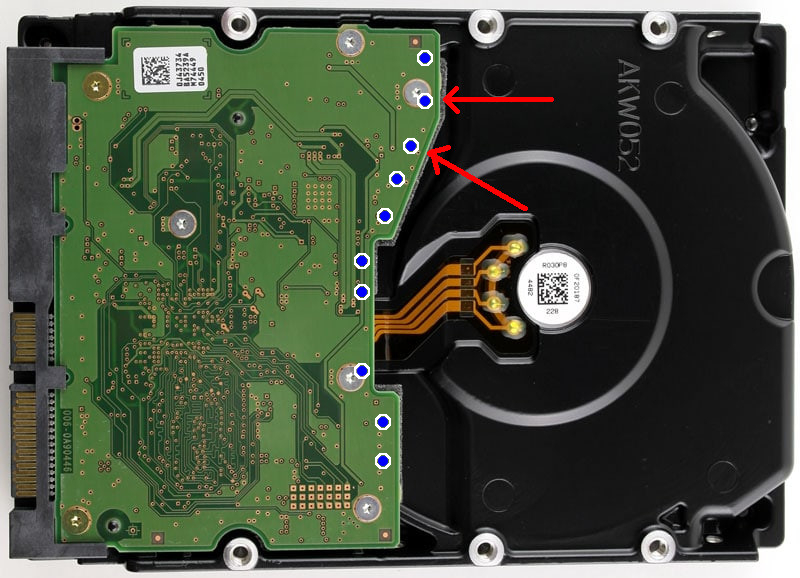
\includegraphics[width=0.45\columnwidth]{hdd-affordances}
	\caption{Affordances in a HDD PCB. Each of the blue
		circles is an affordance for a lever-up action, either for
		removing or loosening the PCB.}
%	\vspace{-1cm}
	\label{fig:hdd-affordances}
\end{figure}

We assume the robot to be equipped with a multifunctional gripper.
This gripper allows performing
bimanual skills with just one manipulator thanks to its two kind
of fingers: a couple of parallel fingers for grasping
and a SCARA finger to assist in grasping or for manipulation of
the device while it is held.
The gripper allows to carry several
tools and has the potential to use them with two grasping modes:
power grab, using all the fingers to perform a stable and powerful grasp;
and the SCARA mode, using the third finger
to grab the tool while the parallel fingers hold the device.

%We assume the robot to be equipped with a multifunctional gripper such as the
%one showed in Fig.~\ref{fig:gripper-kit}. This gripper allows performing
%bimanual skills with just one manipulator thanks to its two kind
%of fingers: a couple of parallel fingers for grasping
%and a SCARA finger to assist in grasping or for manipulation of
%the device while it is held.
%The gripper allows to carry several
%tools and has the potential to use them with two grasping modes:
%power grab, using all the fingers to perform a stable and powerful grasp%
%~\ref{fig:gripper-kit-power}; and the SCARA mode, using the third finger
%to grab the tool while the parallel fingers hold the device%
%~\ref{fig:gripper-kit-scara}.
%
%\begin{figure}[tbhp]
%	\centering
%	\begin{subfigure}[b]{0.8\columnwidth}
%		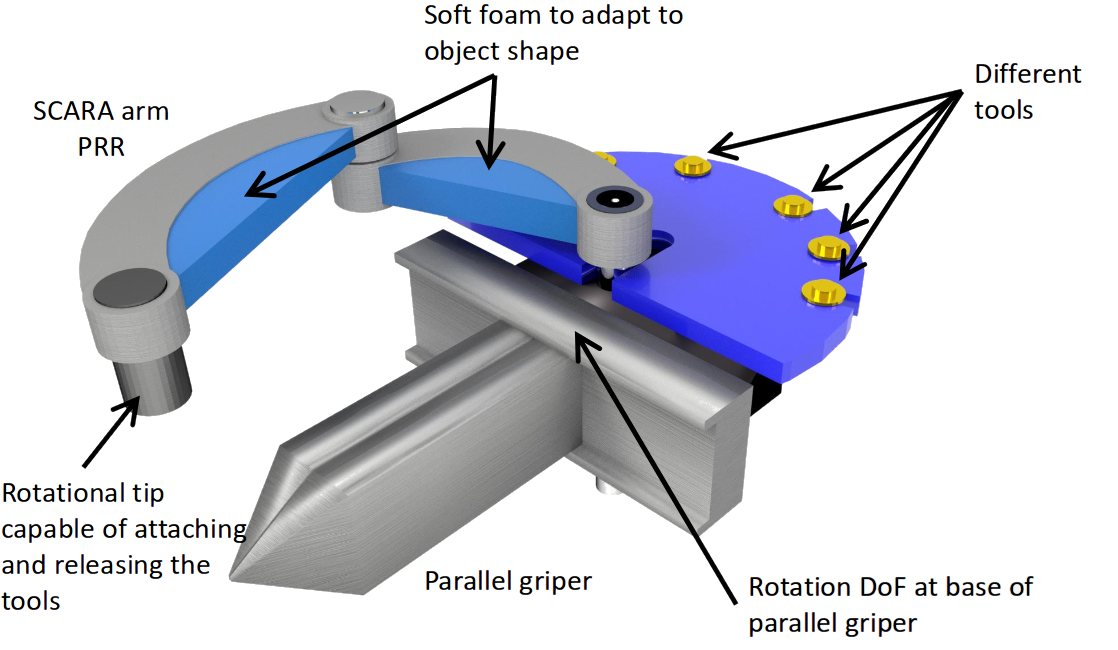
\includegraphics[width=\textwidth]{gripper-kit}
%		\caption{}
%		\label{fig:gripper-kit}
%	\end{subfigure}
%	
%	\begin{subfigure}[b]{0.25\columnwidth}
%		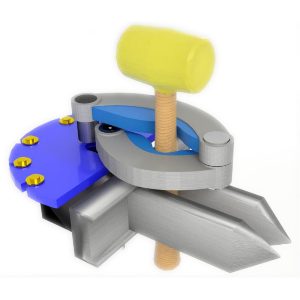
\includegraphics[width=\textwidth]{gripper-kit-power}
%		\caption{}
%		\label{fig:gripper-kit-power}
%	\end{subfigure}
%	\hspace{2cm}
%	\begin{subfigure}[b]{0.25\columnwidth}
%		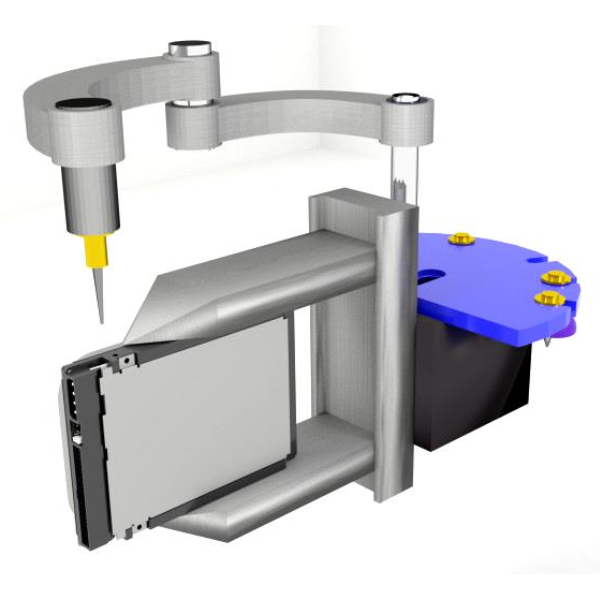
\includegraphics[width=\textwidth]{gripper-kit-scara}
%		\caption{}
%		\label{fig:gripper-kit-scara}
%	\end{subfigure}
%	\caption{
%		(a) Multifunctional gripper designed by KIT (Karlsruher Institut für Technologie) with named parts.
%		(b) Grabbing a hammer with a power grip.
%		(c) Using a tool with the SCARA finger.
%	}
%\end{figure}

All of these considerations have been pondered in order to elaborate a domain that
describes as good as possible the dynamics of a recycling domain. Whether the robot
has equipped one tool, uses a particular mode or is holding the whole device is
critical for planning the next actions. We propose the
following predicates to
describe the robot status and its interaction with the device:
\begin{itemize}
	\item \texttt{(current-mode ?m - mode)}: mode of the currently grasped tool. The
	available modes are \texttt{no-mode} (for when the robot is not grabbing any tool),
	\texttt{scara} and \texttt{power}.
	
	\item \texttt{(current-tool ?t - tool)}: indicates the currently equipped tool. We
	consider the following tools: \texttt{flat-sd} (flat screwdriver), \texttt{star-sd}
	(star screwdriver), \texttt{suction pads}, \texttt{pliers}, a \texttt{hammer} and a \texttt{cuter}.
	
	\item \texttt{(valid-mode ?t - tool ?m - mode)}: indicates that \texttt{?m} is a valid mode
	for tool \texttt{?t}. Some tools like the screwdriver and the suction pad are valid both
	in \texttt{scara} mode and in \texttt{power} mode. However, others like the hammer are valid only
	in power mode.
	
	\item \texttt{(current-side ?s - side)}: the side of the device that is currently facing
	upwards. We assume that the device has a prism-like shape. We consider 6 possible sides:
	\texttt{top}, \texttt{bottom}, \texttt{left}, \texttt{right}, \texttt{front} and
	\texttt{back}. Each component of the device is visible from a specific side (e.g. in a hard
	drive the lever and the platters are at the top, while the PCB is located at the bottom).
	
	\item \texttt{(opposite-side ?s1 ?s2 - side)}: when a particular side is facing upwards, the loosen components at the opposite face fall down. This predicates is used to mark the opposite side
	pairs.
	
	\item \texttt{(held)}: tells whether the device is being held between the parallel fingers.
	This is necessary to flip it over and to perform actions in \texttt{scara} mode.
\end{itemize}

The predicates presented here do not say anything about the configuration of the different components
of the device being recycled. This is covered in the next
Section.

\subsection{Device representation}

While the previous list of predicates is related to
the robot capabilities and its interaction with the
device, we must also encode in the state the information
about the device itself. That is: the detected components
and affordances, the screws, connectors, partial occlusions,
etc.

Below we show a list with the proposed predicates to represent
a device's inner configuration. Fig.~\ref{fig:examples-of-device-predicates}
shows three examples of usage.
\begin{itemize}
	\item \texttt{(at-side ?c - component ?s - side)}: tells the side
	where a certain component is located at. This side has to be facing
	upwards in order to interact with the affordances of this component.
	
	\item \texttt{(broken-component ?c - removable-component)}: the
	component is in such a bad shape that the robot cannot use its
	affordances. This often results in a dead end, unless the component
	is loosen, in which case the device can be turned around in order
	to let it fall.
	
	\item \texttt{(broken-tool ?t - tool)}: the tool is broken
	and it can no longer be used for further manipulation.
	
	\item \texttt{(connected ?c1 ?c2 - component)}: tells that two components
	are connected via a cable or a flat connector.
	
	\item \texttt{(clear ?c - removable-component)}: true for components
	that neither are connected to anything nor have any screw fixing
	them.
	
	\item \texttt{(fixed-by ?c - removable-component ?s - screw)}: true
	for pairs of components-screws in which the screw keeps the component
	in place.
	
	\item \texttt{(has-affordance ?c - removable-component ?a - affordance)}:
	indicates that a component has associated a certain affordance.
	
	\item \texttt{(has-confidence ?a - affordance ?c - affordance-confidence)}:
	indicates the confidence associated to each affordance. We consider
	three levels of confidence: \texttt{low}, \texttt{medium} and
	\texttt{high}.
	
	\item \texttt{(loose ?c - removable-component)}: identifies components
	that are loose and may fall just by turning the device around.
	
	\item \texttt{(partially-occludes ?c1 ?c2 - component)}: marks
	pairs of components in which the first argument occludes the second
	one. This is useful to identify hierarchies.
	
	\item \texttt{(removed-non-verified ?c - removable-component)}:
	identifies components that have been removed, but the robot has not
	checked behind them to see if they were occluding another
	component or affordance.
	
	\item \texttt{(removed-verified ?c - removable-component)}: the
	component has been removed, and the robot has already checked for
	previously hidden components and affordances.
	
	\item \texttt{(stuck ?s - screw)}: the screw is stuck and it is
	more difficult to retrieve it by simply unscrewing.
	
	\item \texttt{(valid-sd ?s - screw ?sd - screwdriver)}: identifies
	which is the valid screwdriver for a certain screw.
\end{itemize}

\begin{figure}[tbhp]
	\centering
	\begin{subfigure}[b]{0.31\columnwidth}
		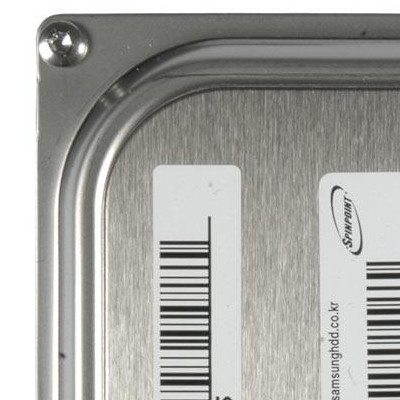
\includegraphics[width=\textwidth]{fixed-by}
		\caption{}
	\end{subfigure}
	~
	\begin{subfigure}[b]{0.31\columnwidth}
		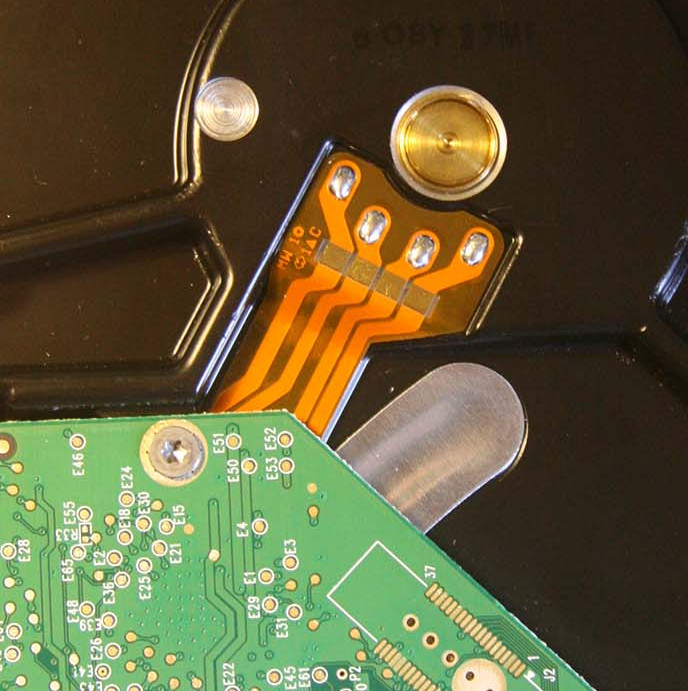
\includegraphics[width=\textwidth]{hdd-conn}
		\caption{}
	\end{subfigure}
	~
	\begin{subfigure}[b]{0.31\columnwidth}
		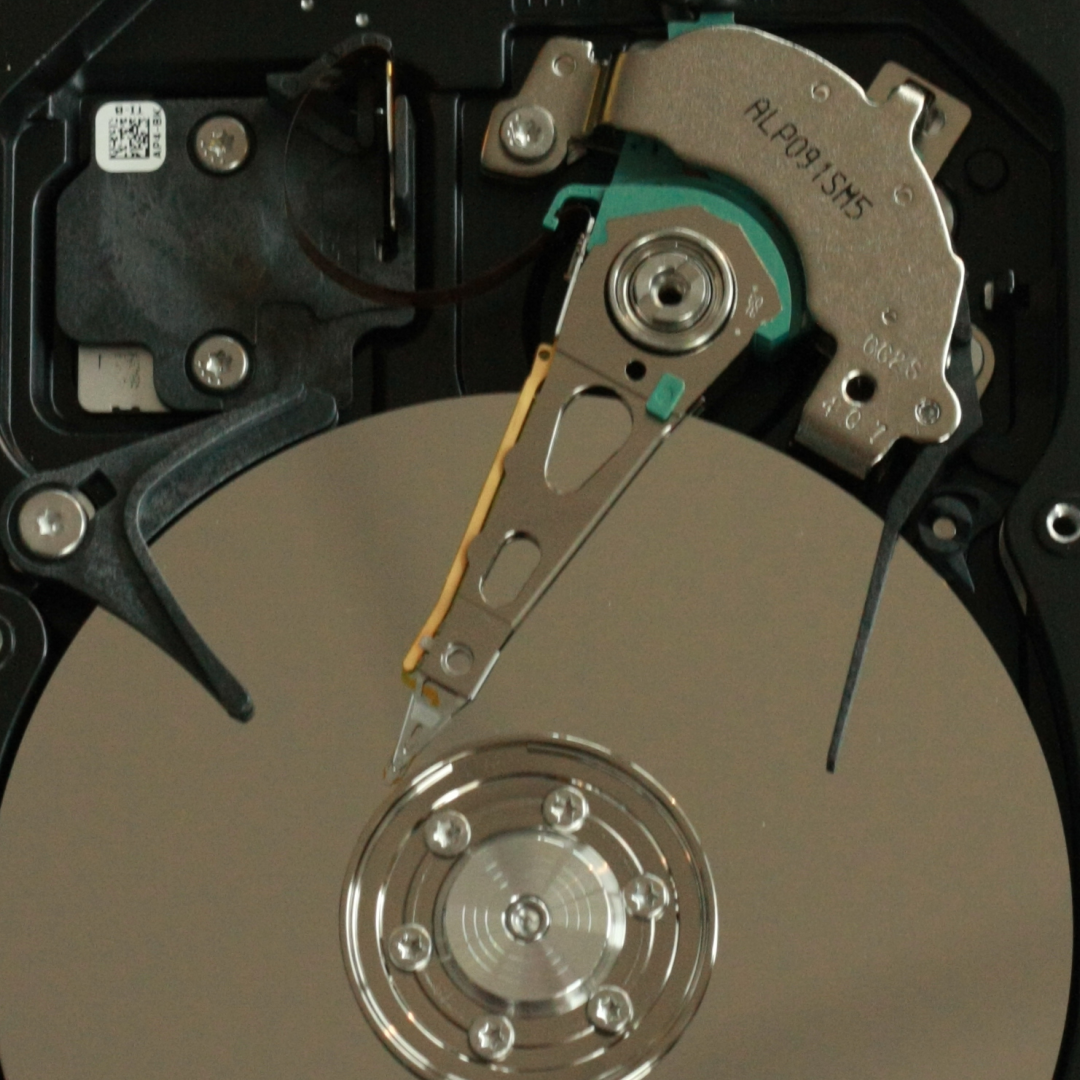
\includegraphics[width=\textwidth]{partially-occluded}
		\caption{}
	\end{subfigure}
	\caption{
		(a) Top lid of a hard drive being fixed by a star screw. If the
		identifiers of the lid and the screw are \texttt{lid} and
		\texttt{lid-s0} respectively, then this would be represented
		as \texttt{(fixed-by lid lid-s0)}.
		(b) Connection between an HDD's PCB and the motor axis. This is
		represented as \texttt{(connected pcb motor-axis)}. Notice that
		this is a symmetric relationship, so the order of the arguments
		may be inverted.
		(c) A hard drive's R/W arm partially occluding a platter.
		Represented as \texttt{(partially-occludes reader platter)}.
		Notice that when one object occludes another, it may as well
		be hiding one of the affordances.
	}
	\label{fig:examples-of-device-predicates}. 
\end{figure}

We consider that these predicates are observable. We assume that we
have a working
perception system that is able to process the scene and
provide them to us, or that there is some middleware to infer them.
We can also think of hidden components and
relationships. These are not observed by the disassembling agent, but the
simulated environment we use for experimentation (see
Chapter~\ref{chap:experimental}) would need to take them into
account since they are part of the ground truth about the device.
They are needed to
identify those components that are not visible (e.g. the disassembling
should not be aware of the components under the HDD lid until the
lid is removed).
\begin{itemize}
	\item \texttt{(hides-component ?c1 ?c2 - component)}: tells that
	the second argument is not visible by the recycling robot because
	it is completely occluded by the first argument component.
	\item \texttt{(hides-affordance ?c1 - component ?a - affordance)}:
	tells that the second argument affordance is completely hidden
	by the first agument component and, therefore, it should not be
	included into the robot's state.
\end{itemize}

\subsection{Actions}

Finally, we will briefly comment on the actions available to the robot.
We have assumed that the actions for picking and placing the device,
switching tools and turning the device around when is held by the robot,
are deterministic. On the other hand, we have modeled several actions
for unscrewing, bashing and retrieve the components with
specialized tools that have probabilistic effects (e.g. successful
retrieval of the object, tool break, component break).

Namely, we have included the following actions in the domain:
\begin{itemize}
	\item \texttt{pick-tool}, \texttt{put-away-tool}, \texttt{grab-device},
	\texttt{place-device}, \texttt{flip}: all of these are deterministic.
	We believe their names to be self-explanatory.
	\item \texttt{let-fall-down}: also deterministic. Produces that all
	the loosened components fall down by virtue of turning the device
	around.
	\item \texttt{cut-connector}: deterministic action for removing
	the \texttt{(connected ?c1 ?c2)} predicate.
	\item four \texttt{unscrew} actions. The probability of
	successfully unscrewing a screw depends on the grasp mode and whether
	the screw is stuck or not (hence the 4 actions).
	\item \texttt{bash} action for quickly remove all the screws that
	are fixing some component, and loosening it. However, it has a low
	success probability and may break the bashed component. This action
	only works with the hammer tool.
	\item six \texttt{lever} actions (all the combinations of modes
	and affordance confidence) for levering a device, each with different
	success/dead-end probabilities.
	\item 3 \texttt{suck-away} actions, each for a different level
	of confidence (the mode does not matter here). This action has a
	very low dead-end probability, but also the success rate (even
	for highly trusted affordances) is low.
	\item 3 \texttt{extract-with-pliers} actions. The pliers are available
	only with the power mode, so the 3 actions correspond to the three
	levels of confidence of the affordance. This action has a very
	high chance of succeeding, but it also has more risk of breaking
	the device than the lever action(s).
\end{itemize}

The complete PPDDL domain specification can be found
in Annex~\ref{chap:ppddl-model}

\IfEq{\jobname}{\detokenize{root}}{}{\printbibliography}

\end{document}